\begin{minipage}{0.75\linewidth}
\begin{figure}[h]
    \centering
    \begin{adjustbox}{max width=1.0\linewidth, keepaspectratio}
        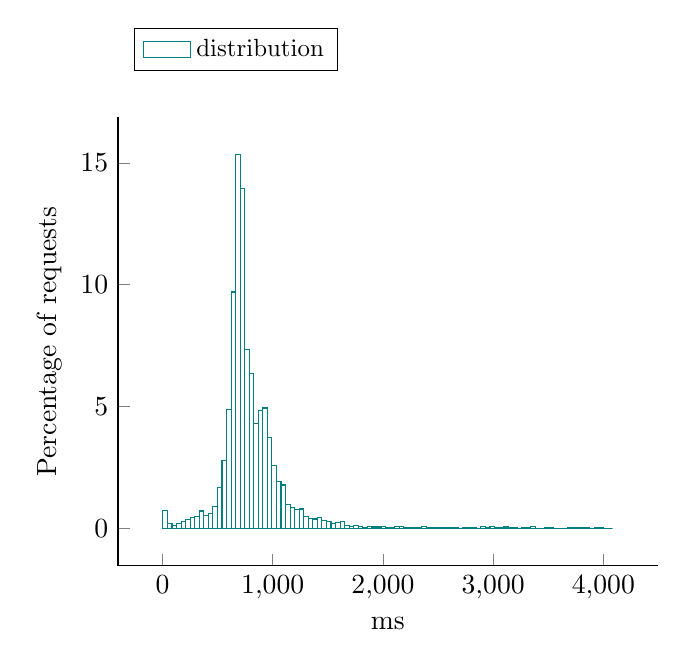
\begin{tikzpicture}
            \begin{axis}[ylabel = Percentage of requests, 
xlabel = ms, 
legend style = {nodes={scale=0.9, transform shape}, at={(0.03,1.2)}, anchor=north west, draw=black, fill=white, align=left, legend columns=3},
area style, mark size = 0pt,
 cycle list name = exotic,
  axis lines* = left]
		\addplot +[ybar interval] coordinates {
			 (4, 0.730004)
			 (45.21, 0.179856)
			 (86.42, 0.126957)
			 (127.63, 0.179856)
			 (168.84, 0.264494)
			 (210.05, 0.370292)
			 (251.26, 0.44435)
			 (292.47, 0.486669)
			 (333.68, 0.708845)
			 (374.89, 0.539568)
			 (416.1, 0.624207)
			 (457.31, 0.878121)
			 (498.52, 1.68218)
			 (539.73, 2.79306)
			 (580.94, 4.86669)
			 (622.15, 9.70165)
			 (663.36, 15.3407)
			 (704.57, 13.9653)
			 (745.78, 7.34236)
			 (786.99, 6.36902)
			 (828.2, 4.30597)
			 (869.41, 4.84554)
			 (910.62, 4.94075)
			 (951.83, 3.73466)
			 (993.04, 2.5603)
			 (1034.25, 1.92552)
			 (1075.46, 1.7774)
			 (1116.67, 0.983919)
			 (1157.88, 0.846382)
			 (1199.09, 0.761744)
			 (1240.3, 0.793483)
			 (1281.51, 0.47609)
			 (1322.72, 0.391452)
			 (1363.93, 0.380872)
			 (1405.14, 0.433771)
			 (1446.35, 0.327973)
			 (1487.56, 0.264494)
			 (1528.77, 0.211595)
			 (1569.98, 0.222175)
			 (1611.19, 0.296234)
			 (1652.4, 0.126957)
			 (1693.61, 0.0846382)
			 (1734.82, 0.126957)
			 (1776.03, 0.0846382)
			 (1817.24, 0.0317393)
			 (1858.45, 0.0846382)
			 (1899.66, 0.0528989)
			 (1940.87, 0.0528989)
			 (1982.08, 0.0846382)
			 (2023.29, 0.0317393)
			 (2064.5, 0.0211595)
			 (2105.71, 0.0740584)
			 (2146.92, 0.0740584)
			 (2188.13, 0.0423191)
			 (2229.34, 0.0211595)
			 (2270.55, 0.0105798)
			 (2311.76, 0.0211595)
			 (2352.97, 0.0634786)
			 (2394.18, 0.0105798)
			 (2435.39, 0.0423191)
			 (2476.6, 0.0211595)
			 (2517.81, 0.0105798)
			 (2559.02, 0.0105798)
			 (2600.23, 0.0211595)
			 (2641.44, 0.0211595)
			 (2682.65, 0)
			 (2723.86, 0.0211595)
			 (2765.07, 0.0317393)
			 (2806.28, 0.0423191)
			 (2847.49, 0)
			 (2888.7, 0.0634786)
			 (2929.91, 0.0211595)
			 (2971.12, 0.0634786)
			 (3012.33, 0.0105798)
			 (3053.54, 0.0211595)
			 (3094.75, 0.0528989)
			 (3135.96, 0.0105798)
			 (3177.17, 0.0211595)
			 (3218.38, 0)
			 (3259.59, 0.0317393)
			 (3300.8, 0.0211595)
			 (3342.01, 0.0634786)
			 (3383.22, 0)
			 (3424.43, 0)
			 (3465.64, 0.0211595)
			 (3506.85, 0.0211595)
			 (3548.06, 0)
			 (3589.27, 0)
			 (3630.48, 0)
			 (3671.69, 0.0423191)
			 (3712.9, 0.0211595)
			 (3754.11, 0.0423191)
			 (3795.32, 0.0211595)
			 (3836.53, 0.0105798)
			 (3877.74, 0)
			 (3918.95, 0.0211595)
			 (3960.16, 0.0105798)
			 (4001.37, 0)
			 (4042.58, 0)
			 (4083.79, 0)
		};
\addlegendentry{distribution};
           \end{axis}
      \end{tikzpicture}
  \end{adjustbox}
  \caption{Response time distribution - req = ReadUser-1}
\end{figure}
\end{minipage}\hfill\begin{minipage}{0.18\linewidth}
\begin{table}[h]
\begin{tabular}{|cc|}
\hline
\textbf{} & \textbf{ms}\\ \hline
 \Xhline{0.005\arrayrulewidth}
min & 4\\
 \Xhline{0.005\arrayrulewidth}
max & 4125\\
 \Xhline{0.005\arrayrulewidth}
mean & 805\\
 \Xhline{0.005\arrayrulewidth}
std & 335\\
\hline
\hline
 \Xhline{0.005\arrayrulewidth}
25th & 665\\
 \Xhline{0.005\arrayrulewidth}
50th & 731\\
 \Xhline{0.005\arrayrulewidth}
75th & 898\\
 \Xhline{0.005\arrayrulewidth}
80th & 937\\
 \Xhline{0.005\arrayrulewidth}
85th & 989\\
 \Xhline{0.005\arrayrulewidth}
90th & 1078\\
 \Xhline{0.005\arrayrulewidth}
95th & 1279\\
 \Xhline{0.005\arrayrulewidth}
99th & 2196\\
\hline
\end{tabular}
\caption{Response time}
\end{table}
\end{minipage}\hfill